\documentclass[a4paper,12pt]{ctexart}     %页面大小和字体大小

\usepackage{ctex}
\usepackage{mathptmx}
\usepackage{amsmath}
\usepackage{url}  % 添加网页
\usepackage{graphicx} %插入图片的宏包
\usepackage{float} %设置图片浮动位置的宏包
\usepackage{subfigure} %插入多图时用子图显示的宏包


\usepackage{booktabs}  % 三线表
\usepackage{longtable}  %设置跨页表格

\usepackage{geometry}
\geometry{left=3.17cm, right=3.17cm, top=2.54cm, bottom=2.54cm}   %页边距

\linespread{1.25}      %设置行距


% 摘要设置  -->设置为4号字
\renewcommand{\abstractname}{\textbf{\songti\zihao{4}摘\quad 要}}
\usepackage{setspace}  %行间距的宏包



% 设置标题
\ctexset{
	section={
		format=\bfseries\zihao{4}\songti
	},
	subsection={
	format=\bfseries\zihao{-4}\songti
	}
}

% 设置目录
\setcounter{tocdepth}{2} %设定目录深度为2,即只显示到二级标题为止

% 设置页码
\usepackage{fancyhdr}
\setcounter{page}{1}  %从第一页开始
\usepackage{lastpage} 
\pagestyle{fancy} % 选用 fancy style % 其余同 plain style
\fancyhf{} % 清空当前设置
%\fancyhead{} %清空所有页眉
\renewcommand{\headrulewidth}{0pt}  %页眉线宽,设为0可以去页眉线
\cfoot{} 
\rfoot{\textbf{\thepage/\pageref{LastPage}}}

% 设置附录
\renewcommand\appendix{\par
	\setcounter{section}{0}
	\setcounter{subsection}{0}
	\gdef\thesection{附录 }%\Alph{section}}
	\gdef\thesubsection{附录\arabic{subsection}.}}


% 设置 表的编号的字体大小	
\usepackage{caption}
\captionsetup{font={small,stretch=1.25},justification=raggedright}


\usepackage{listings}  %添加代码
% 设置代码格式
\RequirePackage{color,xcolor}
% 设置代码的默认样式
\lstset{
	frame=none,% 取消边框
	breaklines=true,% 允许自动断行
	% breakatwhitespace=true,% 使用此命令仅允许在空格处自动断行
	showstringspaces=false,% 不显示字符串中的空格
	basicstyle=\small\ttfamily,% 设置代码基本样式
	flexiblecolumns=true,% 改善字母间距
	keywordstyle=\color{blue},% 设置关键词样式
	stringstyle=\color[rgb]{0.75,0,0.75},% 设置字符串样式
	commentstyle=\songti\color[rgb]{0,0.5,0},% 设置注释样式
	tabsize=4,% 设置制表符缩进
}

% 设置python代码环境
\lstnewenvironment{python}[1][]{
	\lstset{
		language=Python,
		keywordstyle=\color[RGB]{255,119,0},% 设置Keywords样式
		morekeywords={as},% 将特定单词加入Kewords中
		deletekeywords={print},%从 keywords中去除特定单词
		keywordstyle=[2]\color[RGB]{144,0,144},% 设置Builtins样式
		morekeywords=[2]{print},% 将特定单词加入Builtins中
		stringstyle=\color[RGB]{0,170,0},% 设置字符串样式
		commentstyle=\songti\color[RGB]{221,0,0},% 设置注释样式	
		#1
	}
}{}


%===================================================正文从这里开始===============================================================================

\begin{document}\songti\zihao{-4}	
	
	
%	{\zihao{-2}\heiti
%		\title{(选)应用随机过程课程论文\vspace{-4em}}
%		\date{}
%		\maketitle
%	}
%
%	\thispagestyle{fancy} %单独页的页码设置
%	
%	\begin{center}
%		课程号:754.007.201 \quad 时间:2020-2021学年第二学期
%	\end{center}
%	\vspace*{3\baselineskip}
%	\begin{center}\songti\zihao{-2}
%		\textbf{隐式马尔科夫模型(HMM)的随机模拟}
%	\end{center}
%	
%	\begin{center}
%		华光辉 \quad 经济统计1901 \quad 17066003
%	\end{center}
%
%	\vspace*{2\baselineskip}   %空白间距
%
%
%	\begin{spacing}{1.25}

	\begin{abstract}
		隐马尔可夫模型背后的数学是由LEBaum和他的同事开发的。它与早期由RuslanL.Stratonovich提出的最优非线性滤波问题息息相关。在简单的马尔可夫模型(如马尔可夫链),所述状态是直接可见的观察者,因此状态转移概率是唯一的参数。在隐马尔可夫模型中,状态是不直接可见的,但输出依赖于该状态下,是可见的。每个状态通过可能的输出记号有了可能的概率分布。因此,通过一个HMM产生标记序列提供了有关状态的一些序列的信息。隐马尔可夫模型作为一种统计分析模型,创立于20世纪70年代。80年代得到了传播和发展,成为信号处理的一个重要方向,现已成功地用于生物信息学,语音识别,行为识别,文字识别以及故障诊断等领域。也是如今热门的机器学习领域的一个基础模型之一。
		本文首先给出该模型的两个基本假设,然后介绍该模型中的三个基本问题,以及解决三个问题的方法以及原理
		
		\vspace*{1\baselineskip}   %空白间距
		\noindent{\textbf{关键词:}隐马尔可夫模型,前向后向算法 ,EM算法, 维比特算法 }
	\end{abstract}

	
	
	\section{问题与背景}
	
	\subsection{模型背景}
	
	隐马尔科夫模型描述了一个由一个隐藏的马尔科夫链随机生成不可观测的随机状态序列,再由各个状态生成观测,由此产生一个观测随机序列的随机过程。隐藏的马尔科夫链随机生成的状态的序列,称为状态序列,每个状态生成一个观测,而由此产生的观测的随机序列称为观测序列。把序列的每一个位置看作是一个时刻。
	隐马尔科夫模型的过程可以由图\ref{fig:shiyitu}表示。
	
	\vspace*{1\baselineskip}   %空白间距
	
	\begin{figure}[H] %H为当前位置,!htb为忽略美学标准,htbp为浮动图形
		\centering %图片居中
		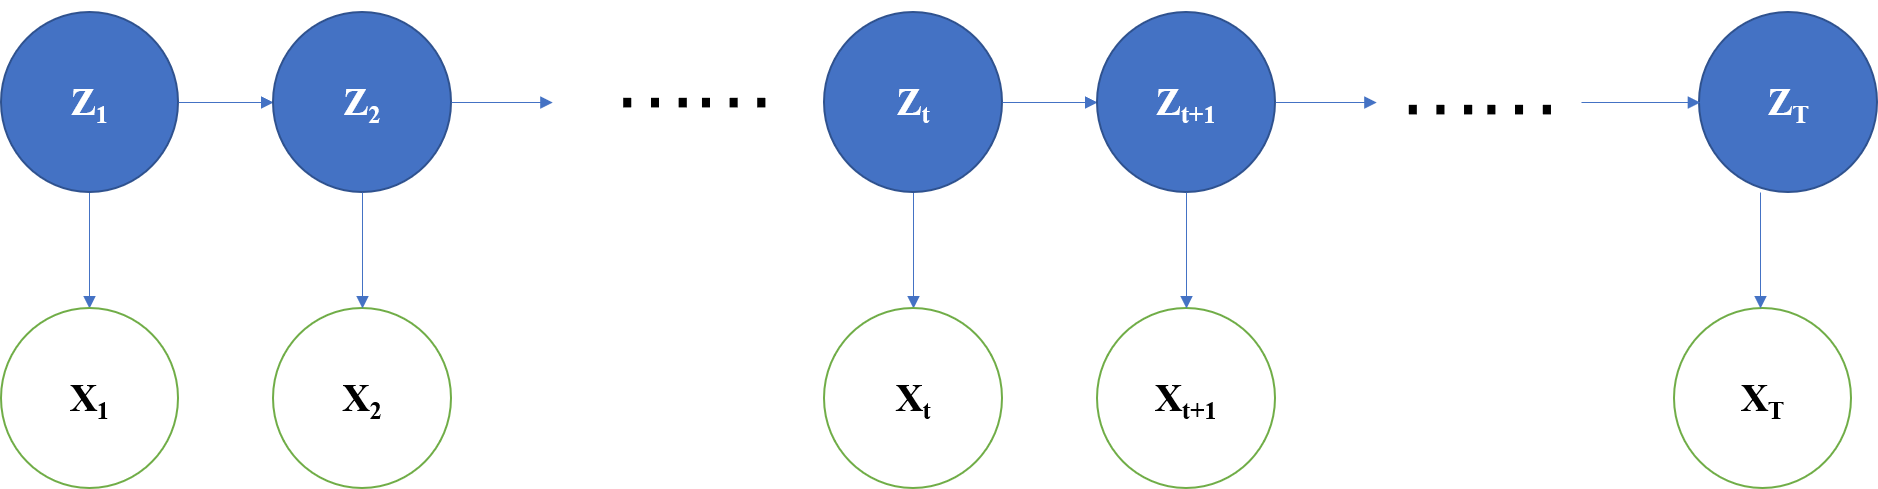
\includegraphics[width=1\textwidth]{示意图.png} %插入图片,[]中设置图片大小,{}中是图片文件名
		\caption{隐马尔科夫模型 \label{fig:shiyitu}} %最终文档中希望显示的图片标题
	\end{figure}
	
	\subsection{问题}
	隐马尔科夫模型有3个基本问题
	
	(1)概率计算问题,给定模型参数$ \lambda = (A,B,\pi) $ 和观测序列 $ O = (o_1,o_2,\dots,o_T) $ 计算观测序列出现的概率 $ P(O|\lambda) $  
	
	(2)参数学习,已知观测序列$ O = (o_1,o_2,\dots,o_T) $ ,估计模型$ \lambda = (A,B,\pi) $ 参数,使得在该模型下观测序列概率 $ P(O|\lambda) $最大,也就是使用极大似然估计的方法估计参数
	
	(3) 预测问题,已知模型参数$ \lambda = (A,B,\pi) $和观测序列$ O = (o_1,o_2,\dots,o_T) $,即对给定观测序列求使得条件概率$ P(I|O) $ 最大的状态序列$ I = (i_1,i_2,\dots,i_T) $
	
	本文将依次给出三个问题的解决办法,最后使用python来模拟状态序列和观测序列生成过程,并对求解进行模拟。
	\section{符号解释}
	

	
\begin{center}
	{\tabcolsep0.25in   % 设置列间距
		\begin{longtable}[htbp]{cc}\songti\zihao{5}
			\renewcommand\arraystretch{1.5}         %表格内部 1.5 倍行距离
			\label{tab:shuoming}\\
			\caption{符号说明 } \\
			\toprule    
			属性 & 符号  \\    
			\midrule 
			所有可能状态的个数 &$ N $ \\
			所有可能观测的个数 & $ M $ \\ 
			状态序列的个数 & $ T $  \\   
			单次状态 & $q_i$ \\ 
			所有可能状态的集合 & $ Q = \{ q_1,q_2,\dots,q_N\} $  \\
			单次观测 & $ v_i $  \\ 
			所有可能观测的集合 & $ V = \{ v_1,v_2,\dots,v_M\} $  \\
			状态序列 & $ I = \{i_1,i_2,\dots,i_T\} $  \\
			观测序列 & $ O = \{ o_1,o_2,\dots,o_T\} $ \\
			状态转移概率 & $ a_{ij} = P(i_{t+1} = q_j | i_t = q_i) $ \\
			条件观测概率 & $ b_j(k) = P(o_t = v_k| i_t = q_j)$ \\ 
			状态转移矩阵 & $ A = [a_{ij} ]_{N \times N} $ \\
			观测矩阵 & $ B = [b_j(k)]_{N \times M} $ \\
			初始状态概率 & $ \pi_i = P(i_1 = q_i)$ \\
			初始状态概率向量 & $ \pi = (\pi_i) $ \\
			所有参数 & $ \lambda = (A,B,\pi) $\\  
			\bottomrule  
			
		\end{longtable} 
	}
\end{center}


	\section{模型假设}
	
	\subsection{齐次马尔科夫假设}
	
	也下一次的隐藏状态只与当前的隐藏状态有关,即马尔科夫性,初始状态由参数$ \pi $决定
	\begin{equation}\label{eq1}
		P(q_{t+1}|q_t,q_{t-1},\dots,q_2,o_t,o_{t_1},\dots,o_1) = P(q_{t+1}|q_t)
	\end{equation}  
	 
	\subsection{独立观测假设}	
	
	\begin{equation}\label{eq2}
	P(o_t|o_{t-1},\dots,o_1,q_t,q_{t-1},\dots,q_1) = P(o_t|q_t)
	\end{equation}


	任意时刻的观测只当前的隐藏状态有关,而与其他任何变量无关
	
	\section{模型求解}
	
		\subsection{概率计算}
		
		给定模型所有参数,即确定了一个隐马尔科夫模型,且给出了观测序列$ O = (o_1,o_2,\dots,o_T) $来计算观测序列$ O $ 出现的概率$ P(O|\lambda) $  
		
		状态序列$ I=(i_1,i_2,\dots,i_T) $出现的概率是
		\begin{equation}
			P(I|\lambda) = \pi_{i_1}a_{i_1i_2}a_{i_2i_3}\dots a_{i_{T-1}i_T}
		\end{equation}
		当状态序列给定之后,我们容易得到观测序列$ O=(o_1,o_2,\dots,o_T) $ 出现的概率
		\begin{equation}
			\begin{split}
				P(O|I,\lambda) &= P(o_t=o_1|i_t=q_{i_1})P(o_t=o_2|i_t=q_{i_2})\dots P(o_t=o_T|i_t=q_{i_T}) \\
				&= b_{i_1}(o_1)b_{i_2}(o_2)\dots b_{i_T}(o_T)
			\end{split}
		\end{equation}
	
	那么对于上述状态序列和一个观测序列同时出现的联合概率为
	\begin{equation} \label{eq3}
		\begin{split}
			P(O|\lambda) &= P(I|\lambda)P(O|I,\lambda)\\
			&= \pi_{i_1}P(o_1|q_{i_1})a_{i_1i_2}P(o_2|q_{i_2})\dots a_{i_{T-1}i_T}P(o_T|q_{i_T})\\
			&= \pi_{i_1}b_{i_1}(o_1)a_{i_1i_2}b_{i_2}(o_2)\dots a_{i_{T-1}i_T}b_{i_T}(o_T)
		\end{split}
	\end{equation}

	但是,利用公式\ref{eq3}计算量很大,每一次至少要计算$ N^T $次,当观测序列较长时,这种算法不可行。下面介绍计算观测序列概率$ P(O|\lambda) $的有效算法:前向-后向算法

			\subsubsection{前向算法}
				给定隐马尔可夫模型及其所有参数,现在定义一个前向概率$ \alpha_t(i) $ ,它表示给定观测序列和在$ t $ 时刻状态的概率,记作
				\begin{equation}
					\alpha_t(i) = P(o_1,o_2,\dots,o_t,i_t=q_i| \lambda)
				\end{equation}
			
				根据这个概率我们可以得到一个$ \alpha_t(i) $ 的初值,
				\begin{equation}
					\alpha_1(i) = \pi_ib_i(o_1)
				\end{equation}
				通过递推我们容易得到
				\begin{equation}
					\begin{split}
						\alpha_{t+1}(i) &= P(o_1,o_2,\dots,o_{t+1},i_{t+1}=q_{t+1}| \lambda) \\
						&= \sum_{i}P(O,I|\lambda)a_{ji}b_i(o_{t+1}) \\
						&= [\sum_{j=1}^{N}\alpha_t(j)a_{ji}]b_i(o_{t+1})
					\end{split}
				\end{equation}
				最后得到
				\begin{equation}
					P(O|\lambda) = \sum_{i=1}^{N}\alpha_T(i)
				\end{equation}
			
				在时刻$ t=1 $,计算$ \alpha_1(i) $的$ N $ 个值;在各个时刻$ t=1,2,\dots,T-1 $ ,计算$ \alpha_{t+1}(i) $的$ N $个值,而且每个$ \alpha_{t+1}(i) $的计算利用前一个时刻$ N $个$ \alpha_t(j) $,这样每一次计算直接引用前一个时刻的结果,避免重复计算。
			\subsubsection{后向算法}
				首先给出向后概率的定义,给定隐马尔科夫模型$ \lambda $,定义在时刻$ t $状态为$ q_i $的条件下,从$ t+1 $ 到$ T $的部分观测序列为$ o_{t+1},o_{t+2},\dots,o_T $的概率为向后概率,记作
			\begin{equation}
				\beta_t(i) = P(o_{t+1},o_{t+2},\dots,o_{T}|i_t = q_i,\lambda)
			\end{equation}
		可以用递推的方法求得向后概率$ \beta_t(i) $以及观测序列概率$ P(O|\lambda) $
		后向算法的具体步骤是首先初始化后向概率,对最终时刻的所有状态规定$ \beta_T(i) =1 $,和前向算法一样,我们得到后向算法的递推公式,对$ t = T-1,T-2,\dots,1 $
		\begin{equation}
			\beta_t(i) = \sum_{i=1}^{N}a_{ij}b_j(o_{t+1})\beta_{t+1}(j)
		\end{equation}
		最终得到概率计算公式
		\begin{equation}
			P(O|\lambda) = \sum_{i=1}^{N}\pi_ib_i(o_1)\beta_1(i)
		\end{equation}
		介绍前向算法和后向算法以后,我们可以得到对于任意的时刻$ t \in {1,2,\dots,T} $有
		\begin{equation}
			P(O|\lambda) = \sum_{i=1}^{N}\sum_{j=1}^{N}\alpha_t(i)a_{ij}b_j(o_{t+1})\beta_{t+1}(j)
		\end{equation}
		\subsection{参数学习}
		如果问题是已知观测序列$ (o_1,o_2,\dots,o_T) $,求待估参数$ \lambda = (A,B,\pi) $,我们很容易想到使用极大似然估计的方法求解待估参数,但是现在出现了隐变量$ I $,我们想要使用极大似然估计必须知道状态序列$ (q_1,q_2,\dots,q_T) $。
		
		根据上面的概率计算问题我们可以知道如果已知隐马尔可夫模型的参数,那么我们容易得到状态序列和观测序列,面对这样的问题,给出$ EM $算法来求解待估参数。
		$ EM $算法的灵魂在于$ Q(\lambda,\bar{\lambda}) $函数,
		\begin{equation}
			\begin{split}
				Q(\lambda,\bar{\lambda}) &= E_I[logP(O,I|\lambda)|O,\bar{\lambda}] \\
				&= \sum_{I}logP(O,I|\lambda)P(O,I|\bar{\lambda})
			\end{split}
		\end{equation}
	
		根据极大似然估计的方法,我们的目标是极大化对数似然函数
		\begin{equation}
			\begin{split}
				L(\lambda) &= log(P(O|\lambda)) \\
				&= log(\sum_{I}P(O|I,\lambda)) \\
				&= log(\sum_{I}P(O|I,\lambda)P(I|\lambda))
			\end{split}
		\end{equation}
	$ Q(\lambda,\bar{\lambda}) $是对数似然函数 $ log(P(O|\lambda)) $在给定观测数据$ O $和当前给定参数$ \bar{\lambda} $对未观测数据$ I $的条件概率分布$ P(O|I,\bar{\lambda}) $的期望。
	
		但是我们并不知道状态序列$ I $,$ EM $的算法的巧妙之处在于我们先给定一个参数$ \bar{\lambda} $,然后利用给定的参数得到$ Q(\lambda,\bar{\lambda}) $,而且我们可以证明的是$ Q(\lambda,\bar{\lambda}) $增长可以保证对数似然函数增长,然后极大化$ Q(\lambda,\bar{\lambda}) $函数,得到新的$ \bar{\lambda} $。
		
		利用新的$ \bar{\lambda} $继续重复上述步骤,同时可以证明$ \bar{\lambda} $会收敛,当$ \bar{\lambda} $不再变化时我们就估计出该隐马尔可夫模型的参数,但是需要注意的是,$ EM $算法的一个缺陷是$ Q(\lambda,\bar{\lambda}) $只能保证对数似然函数局部最优而不能保证全局最优,而且$ \bar{\lambda} $对初值敏感,所以实际情况是我们可以给定不同的初始参数,而后选择最好的那一个。
		
		下面给出使用$ EM $算法的具体步骤来求解隐马尔可夫模型的参数。
		
		$ EM $算法分为$ E $步和$ M $步。
		\paragraph{$ E $步:}
		
		求$ Q(\lambda,\bar{\lambda}) $
		\begin{equation}\label{eq5}
			Q(\lambda,\bar{\lambda})
			= log(\sum_{I}P(O|I,\lambda)P(I|\bar{\lambda}))
		\end{equation}
	根据隐马尔可夫模型的定义得到
	\begin{equation}\label{eq6}
		\begin{split}
			P(O|\lambda) &= P(I|\lambda)P(O|I,\lambda)\\
			&= \pi_{i_1}P(o_1|q_{i_1})a_{i_1i_2}P(o_2|q_{i_2})\dots a_{i_{T-1}i_T}P(o_T|q_{i_T})\\
			&= \pi_{i_1}b_{i_1}(o_1)a_{i_1i_2}b_{i_2}(o_2)\dots a_{i_{T-1}i_T}b_{i_T}(o_T)
		\end{split}
	\end{equation}
	把(\ref{eq6})代入(\ref{eq5})中得到
		\begin{equation}\label{eq7}
				Q(\lambda,\bar{\lambda})
				=\sum_Ilog\pi_{i_1}P(O,I|\bar{\lambda})+\sum_I(\sum_{t=1}^{T-1}loga_{i_ti_{t+1}})P(O,I|\bar{\lambda})+\sum_I(\sum_{t=1}^Tlogb_{i_t}(o_t)P(O,I|\bar{\lambda})	
		\end{equation}
		\paragraph{$ M $步:}
		极大化$ Q $函数$ Q(\lambda,\bar{\lambda}) $求模型参数$ A,B,\pi $
		观察(\ref{eq7}) 可以看出参数单独出现在三项中,所以极大化$ Q(\lambda,\bar{\lambda}) $也就是针对各项极大化即可。
		
		对第一项,
		\begin{equation}
			\sum_Ilog\pi_{i_1}P(O,I|\bar{\lambda})
			= \sum_{i=1}^{N}log\pi_iP(O,i_1 = i|\bar{\lambda})
		\end{equation}
	而且对于初始状态有$ \sum_{i=1}^{N}\pi_i =1$ 
	
	根据拉格朗日乘子法,可以得到
	\begin{equation}
		\pi_i = \frac{P(O,i_1 = i|\bar{\lambda})}{P(O|\bar{\lambda})}
	\end{equation}

	对于第2项可以写成
	\begin{equation}
		\sum_I(\sum_{t=1}^{T-1}loga_{i_ti_{t+1}})P(O,I|\bar{\lambda}) = \sum_{i=1}^{N}\sum_{j=1}^{N}\sum_{t=1}^{T-1}loga_{ij}P(O,i_t=i,i_{t+1} = j|\bar{\lambda})
	\end{equation}

	与计算第1项类似,同时有约束条件$ \sum_{j=1}^{N}a_{ij}=1 $利用拉格朗日乘子法求出
	\begin{equation}
		a_{ij}=\frac{\sum\limits_{t=1}^{T-1}P(O,i_t=i,i_{t+1}=j|\bar{\lambda})}{\sum\limits_{t=1}^{T-1}P(O,i_t=i|\bar{\lambda})}
	\end{equation}

	第3项的计算为
	\begin{equation}
		\sum_I(\sum\limits_{t=1}^{T}logb_{i_t}(o_t))P(O,I|\bar{\lambda}) = \sum\limits_{j=1}^{N}\sum\limits_{t=1}^{T}logb_j(o_t)P(O,i_t=j|\bar{\lambda})
	\end{equation}
	使用同样的方法,约束条件是$ \sum_{k=1}^{M} b_j(k) =1 $,得到
	\begin{equation}
		b_j(k)=\frac{\sum\limits_{t=1}^T,i_t = j|\bar{\lambda}I(o_t=v_k)}{\sum\limits_{t=1}^TP(O,i_t=j|\bar{\lambda})}
	\end{equation}
	最后通过$ EM $算法进行迭代即可估计待估参数
		\subsection{状态解码}
	已知隐马尔可夫模型全部参数$ \lambda $和观测序列$ (o_1,o_2,\dots,o_T) $,求对给定观测序列条件概率$ P(I|O) $最大的状态序列$ I = (i_1,i_2,\dots,i_T) $,求解这个问题的方法称之为维特比算法,实际上是用动态规划的思想求解概率最大路径,这时一条路径对应着一个状态序列。
	
	根据动态规划原理,最优路径具有这样的特性:如果最优路径在时刻$ t $通过结点$ i_t^* $,那么这一路径从结点$ i_t^* $到终点$ i_T^* $的所有可能的部分路径来说,必须是最优的,即部分最优则全局最优。
	
	依据这一原理,我们只需从时刻$ t=1 $开始,递推地计算在时刻$ t $状态为$ i $的各部分路径的最大概率,直至得到时刻$ t=T $状态为$ i $ 的各条路径的最大概率,此时的最大概率即为最优路径的概率,最优路径的终结点也同时得到,然后从最后一个结点开始,由后向前逐步求得结点$ i_{T-1}^*,\dots,i_1^* $,即可求得最优路径。
	\section{模型实例与模拟结果}
		\subsection{生成观测序列}
	采用采用李航老师《统计学习方法》一文中的例子,假设有4个盒子,每个盒子里面都装有红白两种颜色的球,盒子里面的红白球的数量有表\ref{tab:hezi}给出
	
	转移概率矩阵
	
	
	\begin{table}[htbp]\songti\zihao{5} 
		\begin{center}
			\renewcommand\arraystretch{2}         %表格内部 1.5 倍行距离
			\caption{模型数据 \label{tab:hezi}} 
			{\tabcolsep0.3in  %设置列间距
				
				\begin{tabular}{|c|c|c|c|c|}\hline   %开始表格环境,{|c|c|c|}表示文字居中的三列,\hline...\hline表述画两条并排的水平线。
					%\hline必须用于首行之前或者换行命令之后。
					
					\small 盒子编号&1&2&3&4\\\hline   %&是数据分割符号
					红球数&5&3&6&8\\\hline
					白球数&5&7&4&2\\\hline
				\end{tabular}
			}
		\end{center}
	\end{table}
	
	按照下面的方法抽球,产生一个球的颜色的观测序列,开始时以等概率从4个盒子里面选取一个盒子,然后从盒子里面摸一个球,然后再选取一个盒子,只不过下一个盒子并不是等概率选取,而是由于上一个盒子而有不同的概率被选中,其中具体转移概率参看表\ref{tab:zhuanyi},


	
	\begin{center}
		{\tabcolsep0.25in   % 设置列间距
			\begin{longtable}{|c|c|c|c|c|} \caption{\label{tab:zhuanyi}转移概率}\\ \hline\songti\zihao{5}\renewcommand\arraystretch{1.5} %表格内部 1.5 倍行距离
					\small &$ q_1 $ &$ q_2 $&$ q_3 $&$ q_4 $\\\hline   %&是数据分割符号
					$ q_1 $&0&1&0&0\\\hline
					$ q_2 $&0.4&0&0.6&0\\\hline
					$ q_3 $&0&0.4&0&0.6\\\hline
					$ q_4 $&0&0&0.5&0.5\\\hline
			\end{longtable} 
		}
	\end{center}	
	

	不同盒子中由于不同颜色的球的数量并不一样,所以抽到不同颜色的球的概率是不一样的,根据上面的各个盒子中球的数量,我们容易得到不同盒子对应的观测概率如表\ref{tab:shuoming}。  
	
	\begin{table}[htbp]\songti\zihao{5} 
		
		\begin{center}
			\renewcommand\arraystretch{2}         %表格内部 1.5 倍行距离
			\caption{观测概率 \label{tab:guance}} 
			{\tabcolsep0.3in
				
				\begin{tabular}{|c|c|c|}\hline   %开始表格环境,{|c|c|c|}表示文字居中的三列,\hline...\hline表述画两条并排的水平线。
					%\hline必须用于首行之前或者换行命令之后。
					
					\small &$ v_1 $&$ v_2$\\\hline   %&是数据分割符号
					$ q_1 $&0.5&0.5\\\hline
					$ q_2 $&0.3&0.7\\\hline
					$ q_3 $&0.6&0.4\\\hline
					$ q_4 $&0.8&0.2\\\hline
				\end{tabular}
			}
		\end{center}
	\end{table}
	
	
	这就是一个简单的隐马尔可夫模型,毫无疑问,选取盒子的过程就是一个马尔科夫链,我们画出它的概率转移图,如图\ref{fig:zhuanyi}
	\begin{figure}[H] %H为当前位置,!htb为忽略美学标准,htbp为浮动图形
		\centering %图片居中
		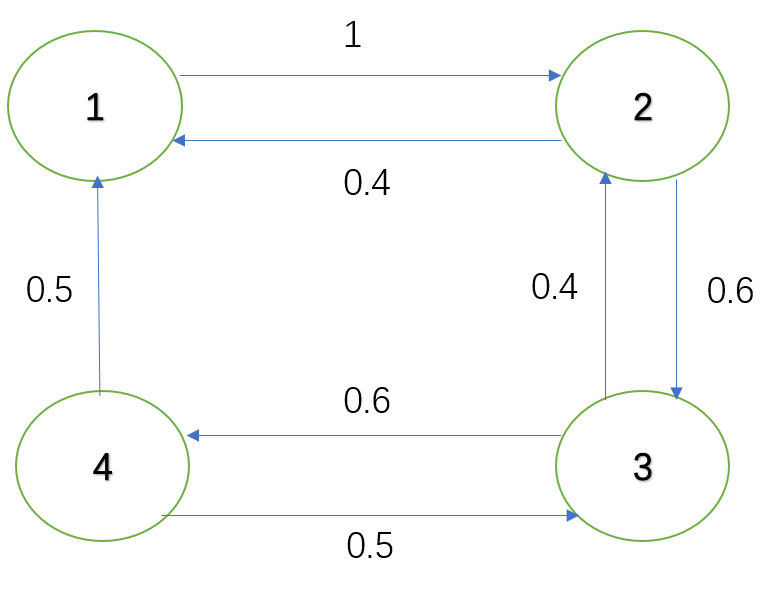
\includegraphics[width=0.51\textwidth]{概率转移图.png} %插入图片,[]中设置图片大小,{}中是图片文件名
		\caption{概率转移图 \label{fig:zhuanyi}} %最终文档中希望显示的图片标题
	\end{figure}

	根据这些参数我们可以生成一个观测序列,而且可以计算任意时刻的观测序列发生的概率。
	
	其步骤可以概括为:
	(1) 按照初始状态分布生成 $ i_1 $
	
	(2) 令  $t=1 $
	
	(3)  按照状态$ i_t $的观测概率分布生成 $ b_{i_t}(k) $生成$ o_t $
	
	(4) 按照状态$ i_t $ 的状态转移概率分布 $ A $ 生成状态 $ i_{+1} $
	
	(5)  令   $ t = t+1 $ 直到$ T $终止
	
	按照这个步骤利用python生成一个10个观测的序列['whiteball', 'whiteball', 'whiteball', 'redball', 'whiteball', 'whiteball', 'whiteball', 'whiteball', 'redball', 'redball']
	
\subsection{计算观测概率和解码问题}
考虑盒子和球模型,$ \lambda = (A,B,\pi) $,状态集合$ Q = \{1,2,3\} $,观测集合$ V =$\{红,白\},

$$A = 
\begin{bmatrix} 
	0.5&0.2&0.3\\
	0.3&0.5&0.2\\ 
	0.2&0.3&0.5
\end{bmatrix} ,\quad
B= 
\begin{bmatrix}
	0.5&0.5\\
	0.4&0.6\\
	0.7&0.3
\end{bmatrix},\quad
\pi = (0.2,0.4,0.4)^T
$$
设$ T=3 $,$ O= $(红,白,红),用前向算法计算$ P(O|\lambda) $
通过定义前向算法函数$ evaluation() $,通过不断迭代求和最终可以得到
$$
P(O|\lambda) = \sum\limits_{i=1}^3\alpha_3(i) = 0.13022
$$
利用后向算法可以算出同样结果 

\subsection{解码问题}
对于$ t=1 $时刻,可以求出状态为$ i $而观测为红球的概率  

在$ t=2 $时,对于每个状态,求出在$ t=1 $时刻状态为$ j $观测为红球而$ t=2 $时刻状态为$ i $而观测为白球的路径的最大概率,比如$ t=2 $时刻若处于$ i=1 $挑选了第一个盒子,则在$ t=1 $时刻有三种可能会使得在$ t=2 $时刻挑选第一个盒子而且摸到白球,分别是第一次选了第一个盒子摸到红球第二次还是第一个盒子摸到白球,另一种可能是第二个盒子红球然后第一个盒子白球,第三个盒子红球第一个盒子白球,保证局部最优,经计算我们保留第三种路径,因为概率最大,且同时保留路径依次迭代下去,可以求得最优状态序列。

通过计算我们求得上述参数下最可能的状态序列是$ \{3,3,3\} $
\subsection{参数学习}
首先我们随机给出一种观察序列(这里设置有4种状态,2种观测),然后根据随机数发生器随机产生10个样本的观测,根据$ EM $算法,求解待估参数。若已知隐马尔可夫模型参数,我们可以生成观测序列,我们通过比较原序列和经过学习后的参数产生的序列对比,检验该算法的有效性。

通过python程序模拟,我们把随机生成的观测序列和经参数产生的序列进行可视化处理,某次结果见图\ref{fig:acc},图中可以看到准确率达到了0.9,
\begin{figure}[H] %H为当前位置,!htb为忽略美学标准,htbp为浮动图形
	\centering %图片居中
	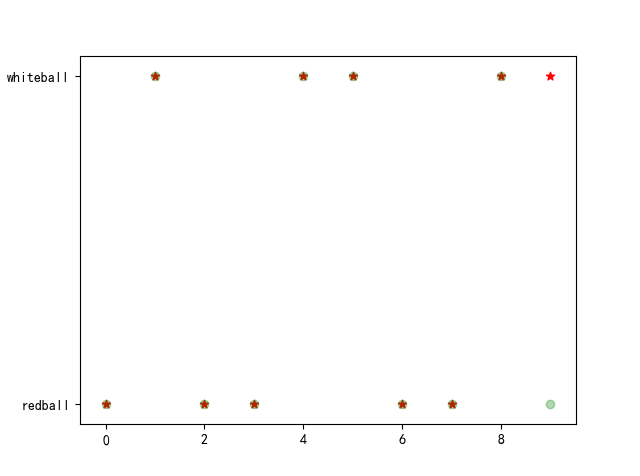
\includegraphics[width=0.7\textwidth]{Figure_1.png} %插入图片,[]中设置图片大小,{}中是图片文件名
	\caption{真实观测与模拟观测 \label{fig:acc}} %最终文档中希望显示的图片标题
\end{figure}

为了寻求该参数学习的有效性,针对每次随机生成的观测都求出其准确率,下面给出简单进行10次模拟的准确率的结果图,如图\ref{fig:accuracy}所示,通过计算机进行了100000次模拟,求这100000次准确率的平均值来表示该参数学习的有效性,经计算得准确率的期望达到了0.82。
\begin{figure}[H] %H为当前位置,!htb为忽略美学标准,htbp为浮动图形
	\centering %图片居中
	\includegraphics[width=0.7\textwidth]{accuracy_1.png} %插入图片,[]中设置图片大小,{}中是图片文件名
	\caption{准确率 \label{fig:accuracy}} %最终文档中希望显示的图片标题
\end{figure}


%================================================================正文结束==========================================================================

	\begin{thebibliography}{99}    %参考文献开始
		\bibitem{1}李航,统计学习方法,北京:清华大学出版社,2012.3。     
		\bibitem{quanjing} Weisong Zhao,HMM隐马尔可夫模型详解,\url{https://blog.csdn.net/weixin_41923961/article/details/82750687},20(3),2021。
		
		
		
		
	\end{thebibliography}

	
	\addcontentsline{toc}{section}{参考文献}
	
	
	
	\begin{appendix}

	\begin{center}
		\section{}
	\end{center}

	
	\subsection{随机模拟程序}
	\begin{python}
#coding=utf-8
#author: Guanghui Hua

import numpy as np
class HMM(object):
	def __init__(self, N, M, pi=None, A=None, B=None):
		self.N = N
		self.M = M
		self.pi = pi
		self.A = A
		self.B = B
	
	def getDistribution(self, dist): 
		r = np.random.rand()  
		for i, p in enumerate(dist):
			if r < p: return i
			r -= p
	
	def generate(self, T: int):
	
		z = self.getDistribution(self.pi)    
		x = self.getDistribution(self.B[z])  
		result = [x]
		for _ in range(T-1):        
			z = self.getDistribution(self.A[z])
			x = self.getDistribution(self.B[z])
			result.append(x)
		for i in range(len(result)):
			if 0 ==result[i]:
			result[i] = "redball"
			else:
			result[i] = "whiteball"
		return result
	
	def evaluate(self, X):
	
		alpha = self.pi * self.B[:,X[0]]
		for x in X[1:]:
			alpha_next = np.empty(self.N)
		for j in range(self.N):
			alpha_next[j] = np.sum(self.A[:,j] * alpha * self.B[j,x])
		alpha = alpha_next
		# alpha = np.sum(self.A * alpha.reshape(-1,1) * self.B[:,x].reshape(1,-1), axis=0)
		return "{:.9f}".format(alpha.sum())
		
	
	def evaluate_backward(self, X):
		beta = np.ones(self.N)
		for x in X[:0:-1]:
			beta_next = np.empty(self.N)
		for i in range(self.N):
			beta_next[i] = np.sum(self.A[i,:] * self.B[:,x] * beta)
		beta = beta_next
		return np.sum(beta * self.pi * self.B[:,X[0]])
		
	def decode(self, X):
		T = len(X) 
		x = X[0]
		delta = self.pi * self.B[:,x]
		varphi = np.zeros((T, self.N), dtype=int)
		path = [0] * T
		for i in range(1, T):
			delta = delta.reshape(-1,1)    
			tmp = delta * self.A
			varphi[i,:] = np.argmax(tmp, axis=0)
			delta = np.max(tmp, axis=0) * self.B[:,X[i]]
		path[-1] = np.argmax(delta)
		for i in range(T-1,0,-1):
			path[i-1] = varphi[i,path[i]]
		return path
	
	def get_something(self, X):
		
		T = len(X)
		alpha = np.zeros((T,self.N))
		alpha[0,:] = self.pi * self.B[:,X[0]]
		for i in range(T-1):
			x = X[i+1]
			alpha[i+1,:] = np.sum(self.A * alpha[i].reshape(-1,1) * self.B[:,x].reshape(1,-1), axis=0)
		
		beta = np.ones((T,self.N))
		for j in range(T-1,0,-1):
			for i in range(self.N):
				beta[j-1,i] = np.sum(self.A[i,:] * self.B[:,X[j]] * beta[j])
		
		return alpha, beta
	def fit(self, X):
	
		self.pi = np.random.sample(self.N)
		self.A = np.ones((self.N,self.N)) / self.N
		self.B = np.ones((self.N,self.M)) / self.M
		self.pi = self.pi / self.pi.sum()
		T = len(X)
		for _ in range(50):
			alpha, beta = self.get_something(X)
			gamma = alpha * beta
		
		for i in range(self.N):
			for j in range(self.N):
				self.A[i,j] = np.sum(alpha[:-1,i]*beta[1:,j]*self.A[i,j]*self.B[j,X[1:]]) / gamma[:-1,i].sum()
		
		for j in range(self.N):
			for k in range(self.M):
				self.B[j,k] = np.sum(gamma[:,j]*(X == k)) / gamma[:,j].sum()
		
		self.pi = gamma[0] / gamma[-1].sum()



def problem1():
	pi = np.array([.25, .25, .25, .25])
	A = np.array([
	[0,  1,  0, 0],
	[.4, 0, .6, 0],
	[0, .4, 0, .6],
	[0, 0, .5, .5]])
	B = np.array([
	[.5, .5],
	[.3, .7],
	[.6, .4],
	[.8, .2]])
	hmm = HMM(4, 2, pi, A, B)
	print(hmm.generate(10))  


def model2():
	def getData(T):   
		data = []
		for _ in range(T):
			x = np.random.choice([0,1])
			data.append(x)#if x <= 1 else 3-x)
		return data
	data = np.array(getData(10))
	data1 = list(data)
	for i in range(len(data1)):
		if 0 ==data[i]:
			data1[i] = "redball"
		else:
			data1[i] = "whiteball"
	hmm = HMM(4, 2)
	hmm.fit(data)               
	gen_obs = hmm.generate(10) 
	t=0
	for i in range(len(data)):
		if data1[i]==gen_obs[i]:
			t+=1
	return t/10
	# x = np.arange(10)
	# plt.scatter(x, gen_obs, marker='*', color='r')
	# plt.scatter(x, data, color='g',alpha=.3)
	# plt.show()
	
def problem2(T):
	lst=[]
	for i in range(T):
		tmp = model2()
		lst.append(tmp)
	# plt.scatter([x for x in range(len(lst))],lst)
	# plt.show()
	return sum(lst)/T


def problem3():
	pi = np.array([.2, .4, .4])
	A = np.array([
	[.5, .2, .3],
	[.3, .5, .2],
	[.2, .3, .5]])
	B = np.array([
	[.5, .5],
	[.4, .6],
	[.7, .3]])
	hmm = HMM(3, 2, pi, A, B)
	print("The probability(forward) of generating an observation sequence is {}".format(hmm.evaluate([0,1,0]))) 
	print("The probability(backward) of generating an observation sequence is {}".format(hmm.evaluate_backward([0,1,0]))) 
	print("The state sequence with the highest probability of generating the observation sequence is{}".format(hmm.decode([0,1,0])))


if __name__ == "__main__":
	problem1()
	problem2(10)
	problem3()

		
\end{python}
	
	\end{appendix}

\end{document}
